\qquad As Tabelas \ref{tab:tempos_quick_v1} e \ref{tab:tempos_quick_v2}
apresentam os tempos de execução, em segundos, obtidos pelas duas
versões do Quick Sort nos seis tamanhos de instância exigidos pelo
trabalho, para cada um dos três tipos de entrada testados. Os valores
são os registrados pelo próprio programa nos arquivos de tempo da
entrega.

\begin{table}[htbp]
    \centering
    \begin{tabular}{|l|r|r|r|r|r|r|}
        \hline
         & 10 & 100 & 1.000 & 10.000 & 100.000 & 1.000.000 \\
        \hline
        Crescente & 0,000001 & 0,000007 & 0,000162 & 0,013770 & 1,346279 & 154,233806 \\
        \hline
        Decrescente & 0,000000 & 0,000003 & 0,000236 & 0,017875 & 1,809272 & 229,408053 \\
        \hline
        Random & 0,000000 & 0,000003 & 0,000036 & 0,000452 & 0,005350 & 0,063731 \\
        \hline
    \end{tabular}
    \caption{Tempo de execução (em segundos) do Quick Sort versão 1 por tamanho e tipo de instância}
    \label{tab:tempos_quick_v1}
\end{table}


\begin{table}[htbp]
    \centering
    \begin{tabular}{|l|r|r|r|r|r|r|}
        \hline
         & 10 & 100 & 1.000 & 10.000 & 100.000 & 1.000.000 \\
        \hline
        Crescente & 0,000004 & 0,000007 & 0,000017 & 0,000137 & 0,001684 & 0,021151 \\
        \hline
        Decrescente & 0,000000 & 0,000001 & 0,000011 & 0,000136 & 0,001716 & 0,022560 \\
        \hline
        Random & 0,000000 & 0,000007 & 0,000075 & 0,000837 & 0,009652 & 0,114290 \\
        \hline
    \end{tabular}
    \caption{Tempo de execução (em segundos) do Quick Sort versão 2 por tamanho e tipo de instância}
    \label{tab:tempos_quick_v2}
\end{table}


\qquad O contraste entre as duas tabelas é o resultado mais importante
deste capítulo. Para 1.000.000 de elementos, a \textbf{versão 1}
levou 154,233806 s na entrada crescente e 229,408053 s na
decrescente, mas apenas 0,063731 s na randômica --- ou seja, a
entrada randômica foi cerca de 2.420 vezes mais rápida que a
crescente e 3.600 vezes mais rápida que a decrescente. A
\textbf{versão 2}, no mesmo tamanho, levou 0,021151 s, 0,022560 s e
0,114290 s, isto é, tempos da mesma ordem de grandeza nas três
situações. Comparando as duas versões nas entradas ordenadas, a
versão 2 foi cerca de \textbf{7.300 vezes} mais rápida na crescente e
\textbf{10.200 vezes} mais rápida na decrescente; na entrada
randômica, ao contrário, a versão 1 foi 1,8 vez mais rápida que a
versão 2 (0,063731 s contra 0,114290 s), porque nesse cenário as duas
já são $O(n \log n)$ e a versão 1 percorre o trecho uma única vez por
partição, enquanto a versão 2 o percorre duas vezes (uma para somar e
outra para trocar).

\qquad Os Gráficos \ref{fig:grafico_quick_v1} e
\ref{fig:grafico_quick_v2} apresentam esses dados em escala linear.
Cada gráfico traz, como pede o enunciado, a curva da entrada já
ordenada (crescente) e a da entrada em ordem decrescente, e também a
da entrada randômica, para completar a comparação. No gráfico da
versão 1, as curvas das duas entradas ordenadas sobem de forma
explosiva, enquanto a curva da entrada randômica fica encostada no
eixo horizontal --- é a assinatura visual do pior caso quadrático
ocorrendo justamente nos dados ordenados. No gráfico da versão 2, as
três curvas ficam abaixo de 0,12 segundo, em uma escala cerca de
duas mil vezes menor.

\begin{figure}[htbp]
    \centering
    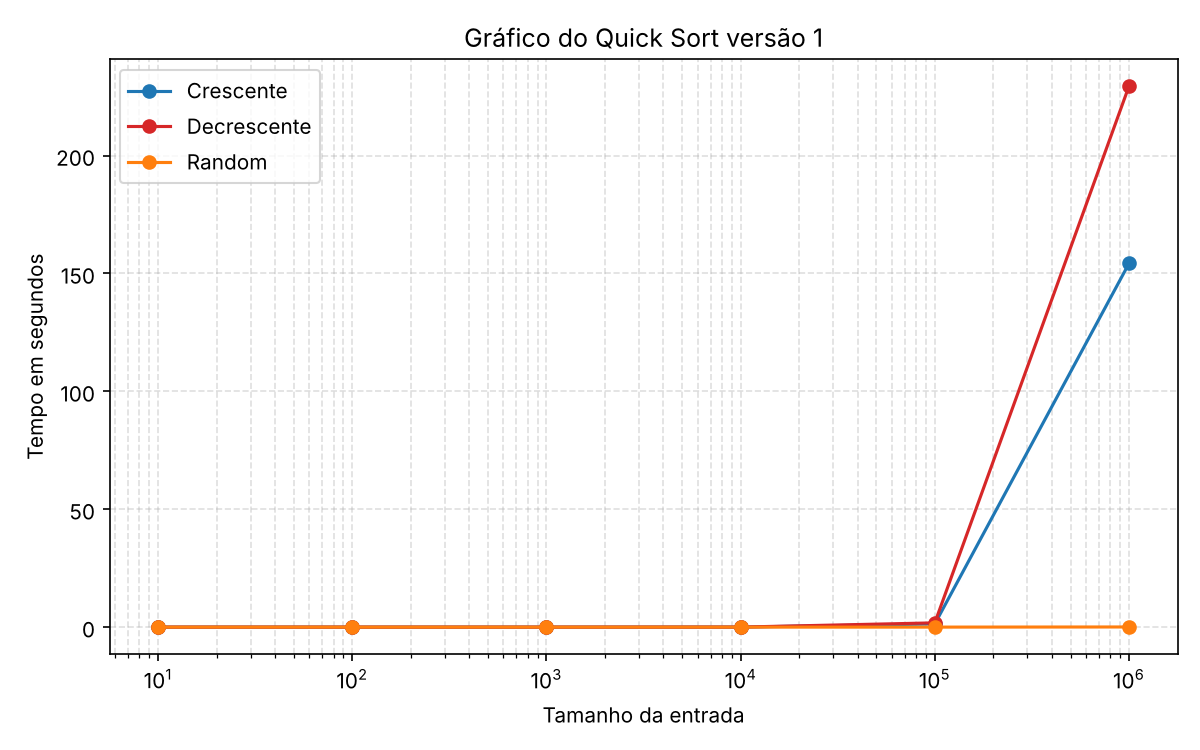
\includegraphics[width=14cm]{Imagens/Quick Sort Versao 1/grafico.png}
    \caption{Gráfico de tempo por tamanho do Quick Sort versão 1 (escala linear)}
    \label{fig:grafico_quick_v1}
\end{figure}

\begin{figure}[htbp]
    \centering
    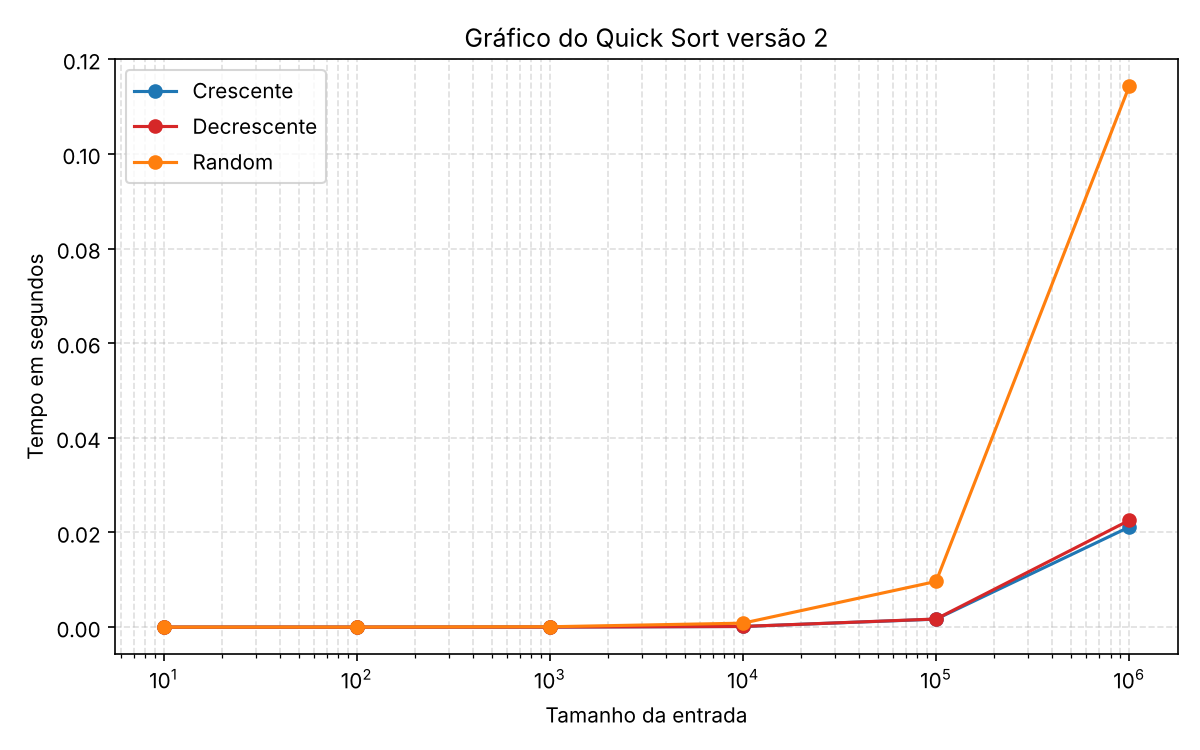
\includegraphics[width=14cm]{Imagens/Quick Sort Versao 2/grafico.png}
    \caption{Gráfico de tempo por tamanho do Quick Sort versão 2 (escala linear)}
    \label{fig:grafico_quick_v2}
\end{figure}

\qquad Os Gráficos \ref{fig:grafico_quick_v1_log} e
\ref{fig:grafico_quick_v2_log} apresentam os mesmos dados em escala
logarítmica nos dois eixos, que permite comparar as taxas de
crescimento: nessa escala, um crescimento quadrático aparece como uma
reta de inclinação 2, e um crescimento da ordem de $n \log n$, como
uma reta de inclinação ligeiramente superior a 1. As duas curvas de
entrada ordenada da versão 1 são visivelmente mais inclinadas que
todas as demais. Os tempos de 0,000000 s (instâncias de 10 elementos,
abaixo da resolução do relógio, de cerca de 1 $\mu$s) não podem ser
representados em escala logarítmica e por isso aparecem como
interrupções no início das curvas.

\begin{figure}[htbp]
    \centering
    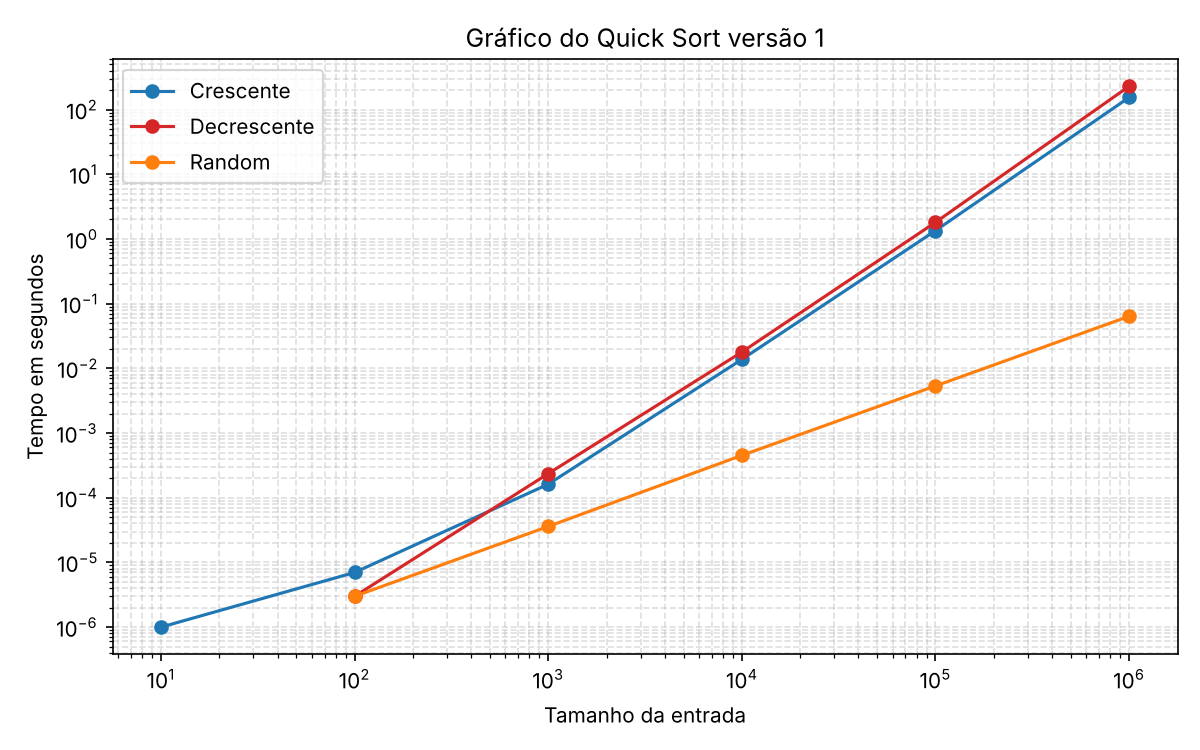
\includegraphics[width=14cm]{Imagens/Quick Sort Versao 1/grafico_log.png}
    \caption{Gráfico de tempo por tamanho do Quick Sort versão 1 (escala logarítmica)}
    \label{fig:grafico_quick_v1_log}
\end{figure}

\begin{figure}[htbp]
    \centering
    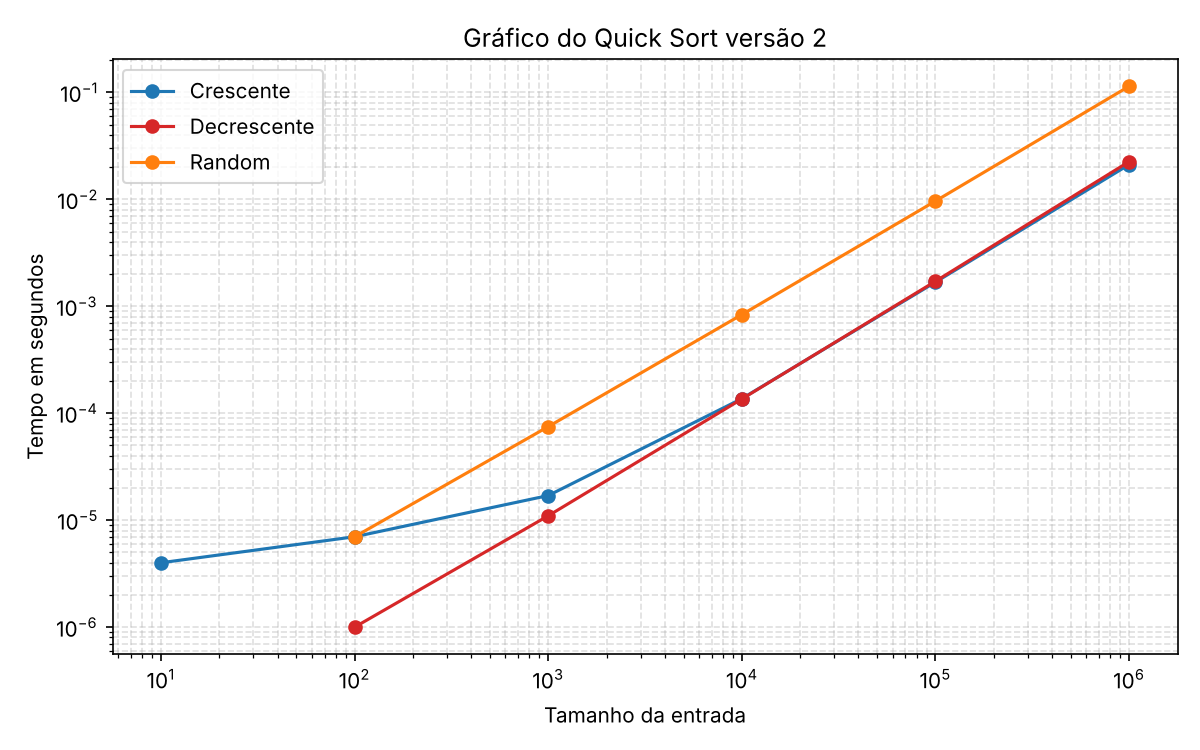
\includegraphics[width=14cm]{Imagens/Quick Sort Versao 2/grafico_log.png}
    \caption{Gráfico de tempo por tamanho do Quick Sort versão 2 (escala logarítmica)}
    \label{fig:grafico_quick_v2_log}
\end{figure}

\qquad Os números confirmam quantitativamente a análise de
complexidade. Multiplicando o tamanho da entrada por 10, de 10.000
para 100.000 elementos, o tempo da versão 1 foi multiplicado por
97,8 (crescente) e 101,2 (decrescente) --- praticamente o fator 100
esperado de um algoritmo quadrático --- e de 100.000 para 1.000.000,
por 114,6 e 126,8, um pouco acima de 100 porque, nesses tamanhos,
o vetor (4 MB) já não cabe na memória \textit{cache} do processador.
Na entrada randômica, o mesmo aumento de 100.000 para 1.000.000
multiplicou o tempo por apenas 11,9, muito próximo de 12,0, que é o
fator esperado para um crescimento $n \log n$ nesse intervalo. A
versão 2 apresentou fatores de 12,6 (crescente), 13,1 (decrescente) e
11,8 (randômica), todos próximos de 12,0: ou seja, a versão 2 é
$n \log n$ nas três situações, exatamente como previsto para um pivô
que divide o trecho em partes equilibradas.

\qquad \textbf{Ambiente de medição.} Os tempos das duas versões do
Quick Sort foram medidos em um ambiente de computação em nuvem, e não
no mesmo computador em que foram medidos os cinco algoritmos dos
capítulos anteriores. O motivo é prático: o pior caso da versão 1 com
1.000.000 de elementos leva vários minutos de processamento contínuo,
o que não foi possível executar no computador pessoal dentro do prazo
de entrega. Para quantificar a diferença entre os dois ambientes, o
Shell Sort e o Merge Sort foram reexecutados no mesmo ambiente de
nuvem, com 1.000.000 de elementos: o Shell Sort levou 0,136953 s na
entrada randômica (contra 0,106033 s no computador pessoal, isto é,
1,29 vez mais lento) e o Merge Sort levou 0,092810 s (contra
0,053426 s, 1,74 vez mais lento). Portanto, \textbf{na tabela de
comparação da próxima seção, diferenças menores que cerca de duas
vezes entre o Quick Sort e os demais algoritmos não devem ser
interpretadas como superioridade de um deles}; as diferenças
relevantes deste trabalho, de três a seis ordens de grandeza,
permanecem válidas.

\qquad Feita essa ressalva, a comparação direta no mesmo ambiente é
favorável ao Quick Sort: para 1.000.000 de elementos em ordem
randômica, a versão 1 (0,063731 s) foi 1,46 vez mais rápida que o
Merge Sort (0,092810 s) e 2,15 vezes mais rápida que o Shell Sort
(0,136953 s), medidos todos no ambiente de nuvem. É esse
comportamento no caso médio, e não o pior caso, que justifica a fama
do Quick Sort como o algoritmo de ordenação interna mais usado na
prática.
